%\documentclass[12pt]{article}
%\documentclass[aip,graphicx,preprint]{revtex4-1}
\documentclass[jkps,preprint,fleqn,showpacs,showkeys]{revtex4}
\RequirePackage{graphicx}
\usepackage{colortbl}
\usepackage[version-1-compatibility]{siunitx}
%\usepackage{ulem}16
\usepackage{amsmath}
\usepackage{amssymb}
\usepackage{amsfonts}
\usepackage{bm}
\usepackage{color}
\usepackage{ulem}
\begin{document}
%\usepackage{amsmath}
%\usepackage{amssymb}
%\usetikzlibrary{positioning, calc}
%\usepackage{tikz}

%\title{review of the paper (Seebeck.., Verma, submitted JLTP)}

%\section*{Title}
%Abstract on knn-assisted transport measurement

\title[]{k-nearest neighbors algorithm-assisted transport measurement}
\author{Nam Kim}
\affiliation{Korea Research Institute of Standards and Science, Daejeon 34113, Republic of Korea}

\date{\today}

\maketitle


\section{Purpose of k-NN algorithm}

The k-nearest neighbours algorithm (k-NN) is used to characterise single-electron pumps.
The concept of a single-electron pump follows the definition of the SI unit of current, the ampere (A)\cite{ampere}.  
One of the advantages of single-electron pumps is their relative accuracy at the level of current magnitude of $10^{-7}$ A. 
The world record of the relative accuracy for this device\cite{stein} is $\sim 2\times 10^{-7}$.
Without the help of k-NN, electron transport measurements for the uncertainty assessment of single electron pumps are time consuming depending on the accuracy level.
However, with the k-NN algorithm, the measurement time can be reduced by about a third.

Typically, the scanning parameters consist of two gate voltages, such as $V_\text{g1}$ and $V_\text{g2}$.
By scanning the parameter space of $V_\text{g1}$ and $V_\text{g2}$, a two-dimensional current density plot can be generated.
The relative accuracy of the single-electron pump is evaluated by analysing the flatness of the current plateau region in the density plot.
The flatness of the plateau is evaluated from the trans-conductance of the current plateau.
Therefore, the programme with the k-NN algorithm performs measurements of the current, $I$ vs $V_\text{g1}$ and $V_\text{g2}$.
 In addition, the measurements of $dI/dV_\text{gi}$ vs $V_\text{g1}$ and $V_\text{g2}$ are also performed,
where $i=1,2$.


\section{measurement results}
We present a preliminary dataset to test the feasibility of our programme.
Using a nonlinear device, we show that the k-NN algorithm is suitable for our purposes.
Fig. 1 describes 3D plot of current $I$ ($z-$axis) vs $V_\text{g1}$ ($x-$axis) and $V_\text{g2}$ ($y-$axis) measured at $T=77$ K. Current and voltage units are nA and V, respectively. 
%V sd=0.1 V, V TR=0.4 V. 
The minus sign of the current is due to the reversed polarity of the current amplifier. 

At this temperatures, the condition $k_\text{B}T > E_\text{C} $ is met, where $E_\text{C} $ denotes the charging energy of the quantum dot. This results in the single-electron pump device, which is composed of the quantum dot, failing to exhibit single-electron transfer phenomena. However, the device demonstrated non-linear characteristics.

\renewcommand{\figurename}{Fig. }
\begin{figure}[h]
\centering
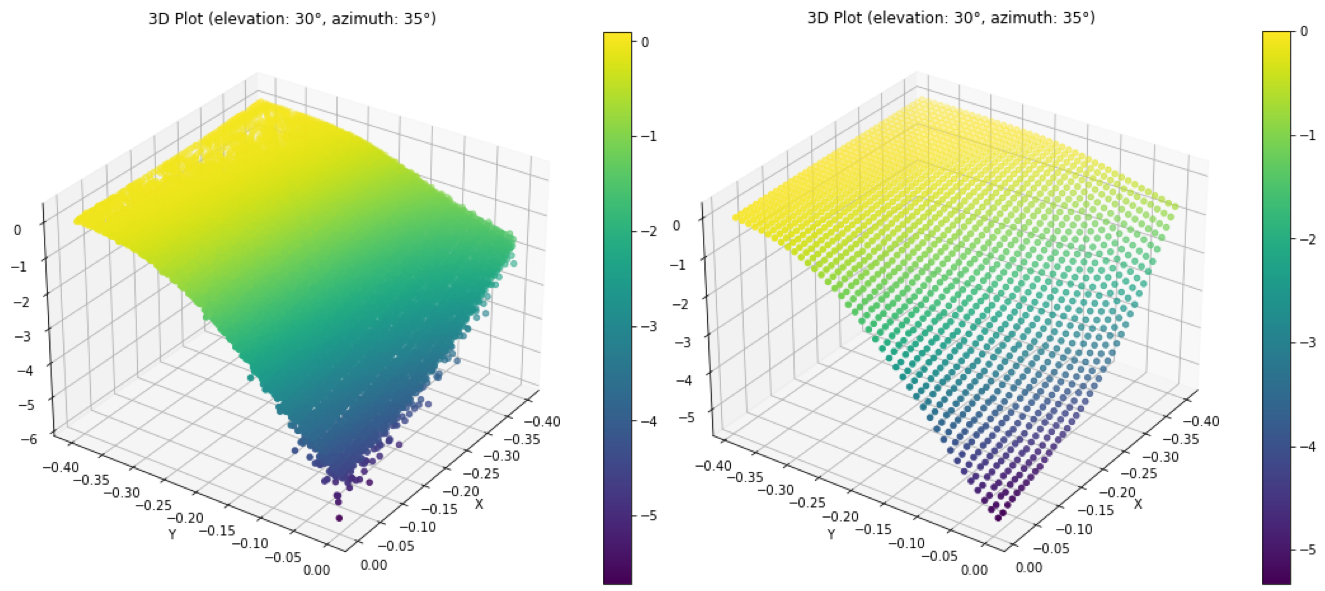
\includegraphics[width=12cm]{Fig_I_Vg}
\parbox{13cm}{\vspace*{0.5cm}
\caption{(Left) k-NN program-created results. The number of data points are 200 by
200. (Right) The number of experimentally measured data points are 40 by 40. 
The number of data points in the left-hand panel is almost three times greater than the number of data points in the right-hand panel. However, the time taken is approximately 60 minutes for both.}
\label{plot1}}
\end{figure}




\begin{thebibliography}{99}
\section*{References}
\bibitem{ampere}
https://www.bipm.org/en/si-base-units/ampere
The ampere, symbol A, is the SI unit of electric current. It is defined by taking the fixed numerical value of the elementary charge e to be $1.602 176 634 x 10^{–19}$ when expressed in the unit C, which is equal to A s, where the second is defined in terms of $\Delta \nu _{Cs}$.

\bibitem{stein}
Stein, F., Drung, D., Fricke, L., Scherer, H., Hohls, F., Leicht, C., Götz, M., Krause, C., Behr, R., Pesel, E. and Pierz, K., 2015. Validation of a quantized-current source with 0.2 ppm uncertainty. Applied Physics Letters, 107(10).


\end{thebibliography}



\end{document}




